%% ใช้ XeLaTeX Compiler
% !TEX program = xelatex
\documentclass[11pt,a4paper]{article}

%% ---- LaTeX syntax utility package ---- %%
\usepackage{etoolbox}

%% ---- Set up paper margin ---- %%
\usepackage[a4paper,top=1in,bottom=1.25in,left=1.25in,right=1in]{geometry}

%% ---- Set up fonts and encoding ---- %%
\usepackage{fontspec}
\usepackage{xunicode}
\usepackage{xltxtra}
\usepackage{gensymb}
\usepackage{comment}


% Enable line breaks for Thai text
\XeTeXlinebreaklocale "th"
\XeTeXlinebreakskip = 0pt plus 2pt minus 1pt

% Set up Thai/Eng fonts
\newfontfamily{\thaifont}{Laksaman}[Scale=MatchLowercase]
\newfontfamily{\englishfont}{CMU Serif}[Scale=MatchLowercase]
\setmainfont{CMU Serif}

\usepackage[Latin, Thai]{ucharclasses}
\setTransitionTo{Thai}{\thaifont}
\setTransitionFrom{Thai}{\englishfont}

%% ---- Load line spacing package ---- %%
\usepackage{setspace}

% Introducing hair space 
\newrobustcmd{\hrsp}{\ifmmode\mskip1mu\else\kern0.0625em\fi}

%% ---- Set up hyperlinks and colors ---- %%
\usepackage{xcolor}
\usepackage[unicode=true]{hyperref}
\hypersetup{%
    colorlinks,%
    linkcolor={red!50!black},%
    citecolor={blue!50!black},%
    urlcolor={blue!80!black},%
}
\renewcommand\UrlFont{\normalfont}
%
\usepackage{physics} % สำหรับพิมพ์เครื่องหมายและสัญลักษณ์ในฟิสิกส์
\usepackage{booktabs}
\usepackage{siunitx} % สำหรับพิมพ์ปริมาณในหน่วย SI
\usepackage{lipsum}
\usepackage{amsmath}
\sisetup{unit-mode = text}% ทำให้พิมพ์สัญลักษณ์ micro และ degree ได้ถูกต้อง
%
\usepackage{tikz} % สำหรับวาด diagram
\usepackage{titling}
%
\newcommand{\subtitle}[1]{%
  \posttitle{%
    \par\end{center}
    \begin{center}\large#1\end{center}
    \vskip0.5em}%
}
\usepackage{multirow} %สำหรับ merge rows

%% ------- Document starts here ------- %%
\begin{document}
%เปลี่ยนเป็นศัพท์ภาษาไทย
\renewcommand{\tablename}{ตารางที่}
\renewcommand{\figurename}{รูปที่}


\title{Laboratory Report of Physics \\ 
	\textbf{Lab: Thermal Expansion}
}
\subtitle{SCPY294 Intermediate Physics Laboratory\\ Department of Physics, Faculty of Science, Mahidol University}

\author{
\textbf{Kritin Wiwatyothin}\\
\\
Teaching Assistant: Withheld for privacy
}

\date{
Experiment conducted: January 2026\\
Report submitted: February 2026
}


\maketitle
\hrule


%% --------------------------------------- %%

\section{บทนำ} \label{introduction}
การทดลองนี้เป็นการศึกษาการขยายตัวเชิงเส้นของโลหะเมื่ออุณหภูมิเปลี่ยนแปลง โดยใช้แท่งโลหะชนิดต่าง ๆ ได้แก่ ทองแดง เหล็กกล้า และอะลูมิเนียม ความยาวที่เปลี่ยนไปของแท่งโลหะจะถูกวัดขณะอุณหภูมิเปลี่ยนแปลงจากความร้อนของไอน้ำ ข้อมูลที่ได้จะนำมาวิเคราะห์เพื่อหาค่าสัมประสิทธิ์การขยายตัวเชิงเส้นของโลหะแต่ละชนิด และเปรียบเทียบกับค่ามาตรฐาน

\subsection*{วัตถุประสงค์} \label{objective}
\begin{enumerate}
    \item เพื่อศึกษาผลของความร้อนต่อการขยายตัวแบบเชิงเส้นของโลหะ
    \item เพื่อหาค่าสัมประสิทธิ์การขยายตัวเชิงเส้นของโลหะตัวอย่าง ได้แก่ ทองแดง เหล็กกล้า และอะลูมิเนียม
\end{enumerate}

\subsection*{ทฤษฎี} \label{theory}

การขยายตัวเชิงเส้น (Linear Expansion) คือการที่วัตถุมีการเปลี่ยนแปลงความยาวในทิศทางเดียวเมื่ออุณหภูมิเปลี่ยนแปลง ซึ่งพบได้ชัดเจนในวัตถุที่มีลักษณะเป็นแท่งหรือเส้น จากการทดลองพบว่าความยาวที่เปลี่ยนไป ($\Delta L$) แปรผันตรงกับความยาวเดิมของวัตถุ ($L_0$) และการเปลี่ยนแปลงของอุณหภูมิ ($\Delta T$) ดังสมการ \cite{Halliday}
\begin{equation}
    \Delta L = \alpha L_0 \Delta T \label{Linear Expansion}
\end{equation}
โดยที่ $\alpha$ คือสัมประสิทธิ์การขยายตัวเชิงเส้นของวัสดุ ซึ่งเป็นสมบัติเฉพาะของวัสดุแต่ละชนิด มีหน่วยเป็น $\text{°C}^{-1}$

เมื่อจัดรูปสมการใหม่ จะสามารถใช้ในการคำนวณค่าสัมประสิทธิ์การขยายตัวเชิงเส้นได้ดังนี้
\begin{equation}
    \alpha = \frac{\Delta L}{L_0 \Delta T} \label{alpha}
\end{equation}

ในการทดลองนี้ ความยาวที่เปลี่ยนไปของแท่งโลหะจะถูกวัดด้วย Dial Gauge ขณะที่อุณหภูมิของโลหะเปลี่ยนแปลง ซึ่งวัดด้วย Thermistor จากนั้นนำข้อมูล $\Delta L$ และ $\Delta T$ มาสร้างกราฟความสัมพันธ์ที่เหมาะสมเพื่อหาค่า $\alpha$ ของโลหะตัวอย่าง และเปรียบเทียบกับค่ามาตรฐาน

\bigskip
\noindent
\textbf{การแปลงค่าความต้านทานของ Thermistor เป็นอุณหภูมิ} \\

ในการทดลองนี้ อุณหภูมิของแท่งโลหะถูกวัดโดยใช้ Thermistor ซึ่งเป็นอุปกรณ์ที่มีค่าความต้านทานเปลี่ยนแปลงตามอุณหภูมิ ความสัมพันธ์ระหว่างค่าความต้านทาน ($R$) และอุณหภูมิ ($T$) ของ Thermistor เป็นความสัมพันธ์ไม่เชิงเส้น (Non-linear) และเพื่อให้ได้ค่าอุณหภูมิที่แม่นยำ การทดลองนี้ใช้สมการ Steinhart--Hart ในการอธิบายความสัมพันธ์ระหว่างค่าความต้านทานของ Thermistor และอุณหภูมิ ดังสมการ ดังสมการ \cite{SteinhartHart}
\begin{equation}
    \frac{1}{T} = A + B \ln R + C (\ln R)^3 \label{SH}
\end{equation}
โดยที่ $T$ คืออุณหภูมิในหน่วยเคลวิน ($\mathrm{K}$), $R$ คือค่าความต้านทานของ Thermistor และ $A$, $B$, และ $C$ เป็นค่าคงที่ของ Thermistor ซึ่งหาได้จากการทำ Curve Fitting

ค่าคงที่ $A$, $B$ และ $C$ ถูกหาจากการฟิตข้อมูลความสัมพันธ์ระหว่างค่าความต้านทานและอุณหภูมิที่ให้มาในตารางมาตรฐานของ Thermistor โดยใช้วิธี Curve Fit จากนั้นจึงนำสมการ Steinhart--Hart ที่ได้ไปใช้คำนวณอุณหภูมิของโลหะจากค่าความต้านทานที่วัดได้จริงในระหว่างการทดลอง





%% --------------------------------------- %%
\section{ขั้นตอนการทดลอง} \label{procedure}

\subsection*{ตอนที่ 1: การเตรียมอุปกรณ์และการตั้งค่าเริ่มต้น}
ในส่วนนี้มีวัตถุประสงค์เพื่อเตรียมชุดทดลองและตั้งค่าพารามิเตอร์เริ่มต้นที่จำเป็นต่อการวัดการขยายตัวเชิงเส้นของโลหะ โดยมีขั้นตอนดังนี้:
\begin{enumerate}
    \item ตรวจสอบความเรียบร้อยของชุดการทดลองการขยายตัวเชิงเส้นของโลหะ และเลือกแท่งโลหะตัวอย่างชนิดทองแดง ติดตั้งเข้ากับฐานรองรับ
    \item ปรับตำแหน่ง Dial Gauge ให้สัมผัสกับแผ่นวัดให้เรียบร้อย
    \item ติดตั้ง Thermistor ให้สัมผัสกับแท่งโลหะเพื่อใช้วัดอุณหภูมิ และต่อมัลติมิเตอร์สำหรับอ่านค่าความต้านทาน
    \item ต่อท่อยางจากแหล่งกำเนิดไอน้ำเข้ากับช่องนำไอน้ำเข้าสู่แท่งโลหะ และตรวจสอบความแน่นหนา
    \item วัดและบันทึกค่าความยาวเริ่มต้นของแท่งโลหะ ($L_0$) ซึ่งกำหนดให้มีค่า 700 mm
\end{enumerate}

\subsection*{ตอนที่ 2: การให้ความร้อนและการวัดการขยายตัวของโลหะ}
ในส่วนนี้มีวัตถุประสงค์เพื่อวัดการเปลี่ยนแปลงความยาวของแท่งโลหะเมื่ออุณหภูมิเปลี่ยนแปลง โดยมีขั้นตอนดังนี้:
\begin{enumerate}
    \item เปิดแหล่งกำเนิดไอน้ำเพื่อให้ไอน้ำไหลผ่านแท่งโลหะ
    \item เมื่ออุณหภูมิของโลหะเพิ่มขึ้นจนใกล้คงที่ ให้บันทึกค่าความต้านทานของ Thermistor และค่าการเปลี่ยนแปลงความยาวของแท่งโลหะ
    \item เมื่อเข็มของ Dial Gauge หยุดนิ่ง แสดงว่าแท่งโลหะอยู่ในสภาวะสมดุลความร้อน ให้ปรับ Dial Gauge มีค่าเริ่มต้นเป็นศูนย์มิลลิเมตร
    \item ปิดการไหลของไอน้ำโดยใช้ตัวล็อคท่อยาง และปล่อยให้แท่งโลหะเย็นตัวลงตามธรรมชาติ
    \item ระหว่างการเย็นตัว ให้บันทึกค่าความต้านทานของ Thermistor และค่าความยาวจาก Dial Gauge ที่อุณหภูมิต่าง ๆ โดยกำหนดจำนวนจุดข้อมูลที่เหมาะสม
\end{enumerate}

\subsection*{ตอนที่ 3: การวิเคราะห์อุณหภูมิและการทำซ้ำการทดลอง}
ในส่วนนี้มีวัตถุประสงค์เพื่อเตรียมข้อมูลสำหรับการวิเคราะห์และเปรียบเทียบผลการทดลอง โดยมีขั้นตอนดังนี้:
\begin{enumerate}
    \item แปลงค่าความต้านทานของ Thermistor ที่วัดได้เป็นค่าอุณหภูมิ โดยใช้วิธี Curve Fitting เข้ากับสมการ Steinhart--Hart จากข้อมูลในตารางรูปที่ \ref{Temp-Res} โดยผลจากการทำ Non-linear Least Squares Fitting ด้วยโปรแกรม \texttt{Python} จะได้ว่า
    \begin{equation}
    \frac{1}{T} = (8.546 + 2.047 \ln R + 9.358 \cross 10^{-4} (\ln R)^3) \cross 10^{-4}
\end{equation}
โดยที่ค่าความคาดเคลื่อนของ T ในสมการนี้จะเท่ากับ $\sigma_{SH} = 0.2$ \celsius
\newline
\textbf{\underline{หมายเหตุ}} T ในสมการยังคงมีหน่วยเป็นเคลวิน (K)
    \item สร้างกราฟความสัมพันธ์ระหว่างการเปลี่ยนแปลงความยาวของแท่งโลหะ ($\Delta L$) กับการเปลี่ยนแปลงอุณหภูมิ ($\Delta T$)
    \item หาค่าสัมประสิทธิ์การขยายตัวเชิงเส้น ($\alpha$) ของโลหะจากความชันของกราฟ
    \item ทำการทดลองซ้ำโดยเปลี่ยนแท่งโลหะเป็นเหล็กกล้าและอะลูมิเนียม ตามลำดับ และวิเคราะห์ผลในลักษณะเดียวกัน
    \item เปรียบเทียบค่าที่ได้จากการทดลองกับค่ามาตรฐานของโลหะแต่ละชนิด
\end{enumerate}

\begin{figure}[htbp]
	\centering
	\makebox[\textwidth]{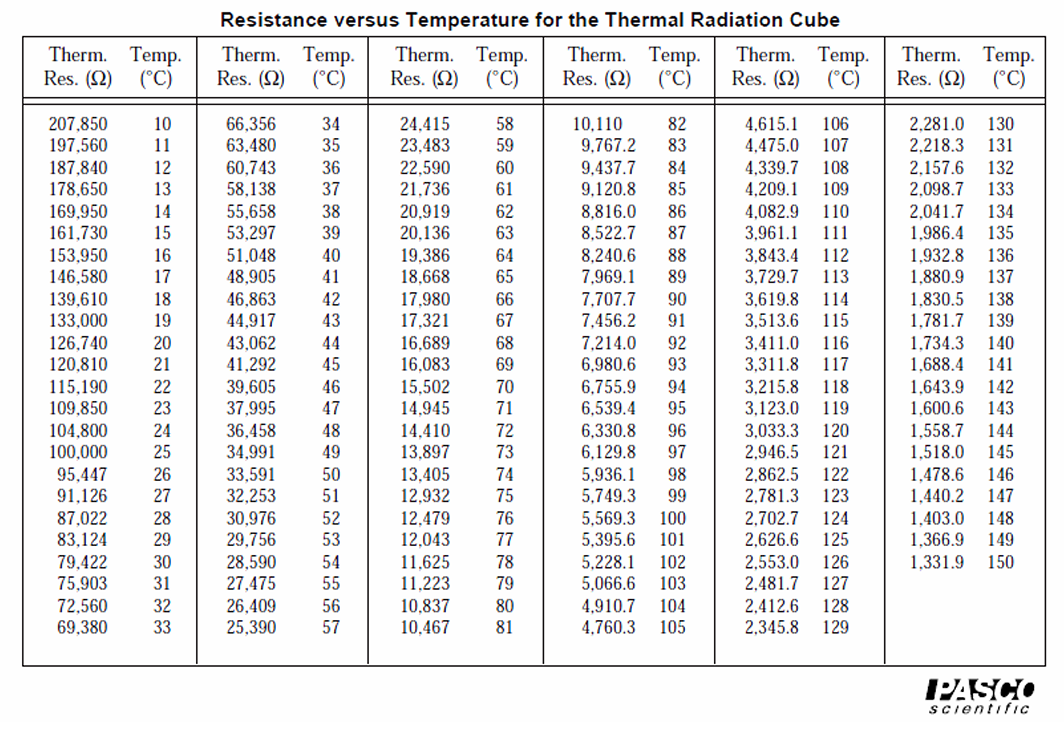
\includegraphics[width=1.1\textwidth]{Thermister_Temp.PNG}}
	\caption{ความสัมพันธ์ระหว่างค่าความต้านทานและอุณหภูมิของ Thermister}
	\label{Temp-Res}
\end{figure}




%% --------------------------------------- %%
\newpage
\section{ผลการทดลอง} \label{result}

\subsection{ข้อมูลจากการทดลอง} \label{data}
จากการทดลอง กำหนดให้ $L_0= 700 \pm 1$ mm และค่าความคาดเคลื่อนของความต้านทานคำนวณได้จาก Manual ที่อุปกรณ์ให้มา นอกจากนี้ยังมีค่าความคลาดเคลื่อนของ Model อุณหภูมิของแท่งโลหะที่ \mbox{$\sigma_{SH} = 0.2$ \celsius} ดังที่กล่าวไป อีกทั้งยังมีความคลาดเคลื่อนจากสเกลของ Dial gauge ซึ่งมีค่าเท่ากับ \mbox{$\sigma_{L_i} = 0.01$ mm}

\bigskip
นอกจากนี้แล้วในการทดลองยังมีการใช้จุดเทียบที่แตกต่างกันสำหรับโลหะแต่ละชนิด โดยจุดเทียบของทองแดง เหล็กกล้า และอะลูมิเนียม จะเป็นจุดที่ $R_c= 12$ k\ohm, $R_s = 10$ k\ohm, และ $R_a = 12$ k\ohm \space ตามลำดับ
จากการทดลองได้ตารางข้อมูลดังนี้

\begin{table}[htbp]
\centering
\caption{ข้อมูลระยะยืดที่วัดได้ ($\Delta L$) และความต้านทานของ Thermistor ($R$) ของทองแดง}
\renewcommand{\arraystretch}{1.2}
\begin{tabular}{|c|ccc|c|c|}
\hline
จุดที่ 
& \multicolumn{3}{c|}{$\Delta L$ ($\pm 0.01$ mm)} 
& $\Delta \bar L$ (mm)
& $R$ (k$\Omega$) \\
\cline{2-4}
& ครั้งที่ 1 & ครั้งที่ 2 & ครั้งที่ 3 & & \\
\hline
1 & 0.13 & 0.16 & 0.14 & 0.14 $\pm$ 0.02 & 15.5 $\pm$ 0.3 \\
2 & 0.21 & 0.22 & 0.21 & 0.21 $\pm$ 0.01 & 18.6 $\pm$ 0.3 \\
3 & 0.30 & 0.29 & 0.28 & 0.29 $\pm$ 0.02 & 22.3 $\pm$ 0.4 \\
4 & 0.36 & 0.35 & 0.34 & 0.35 $\pm$ 0.02 & 26.5 $\pm$ 0.4 \\
5 & 0.42 & 0.41 & 0.40 & 0.41 $\pm$ 0.02 & 31.3 $\pm$ 0.5 \\
6 & 0.45 & 0.44 & 0.43 & 0.44 $\pm$ 0.02 & 35.1 $\pm$ 0.5 \\
7 & 0.49 & 0.47 & 0.46 & 0.47 $\pm$ 0.02 & 39.0 $\pm$ 0.5 \\
8 & 0.52 & 0.51 & 0.49 & 0.51 $\pm$ 0.02 & 43.5 $\pm$ 0.5 \\
9 & 0.54 & 0.53 & 0.52 & 0.53 $\pm$ 0.02 & 47.0 $\pm$ 0.6 \\
\hline
\end{tabular}
\end{table}


\begin{table}[htbp]
\centering
\caption{ผลการคำนวณอุณหภูมิ ($T$) และอุณหภูมิที่เปลี่ยนแปลง ($\Delta T$) ของทองแดง}
\renewcommand{\arraystretch}{1.2}
\begin{tabular}{|c|c|c|c|c|}
\hline
จุดที่ 
& $\Delta \bar L$ (mm)
& $R$ (k$\Omega$)
& $T$ ($^\circ$C)
& $\Delta T$ ($^\circ$C) \\
\hline
1 & 0.14 $\pm$ 0.02 & 15.5 $\pm$ 0.3 & 70.05 $\pm$ 0.6 & 7.1 $\pm$ 0.9 \\
2 & 0.21 $\pm$ 0.01 & 18.6 $\pm$ 0.3 & 65.15 $\pm$ 0.5 & 12.0 $\pm$ 0.9 \\
3 & 0.29 $\pm$ 0.02 & 22.3 $\pm$ 0.4 & 60.39 $\pm$ 0.5 & 16.7 $\pm$ 0.9 \\
4 & 0.35 $\pm$ 0.02 & 26.5 $\pm$ 0.4 & 55.97 $\pm$ 0.4 & 21.2 $\pm$ 0.8 \\
5 & 0.41 $\pm$ 0.02 & 31.3 $\pm$ 0.5 & 51.80 $\pm$ 0.4 & 25.3 $\pm$ 0.8 \\
6 & 0.44 $\pm$ 0.02 & 35.1 $\pm$ 0.5 & 48.98 $\pm$ 0.4 & 28.1 $\pm$ 0.8 \\
7 & 0.47 $\pm$ 0.02 & 39.0 $\pm$ 0.5 & 46.42 $\pm$ 0.4 & 30.7 $\pm$ 0.8 \\
8 & 0.51 $\pm$ 0.02 & 43.5 $\pm$ 0.5 & 43.81 $\pm$ 0.4 & 33.3 $\pm$ 0.8 \\
9 & 0.53 $\pm$ 0.02 & 47.0 $\pm$ 0.6 & 41.98 $\pm$ 0.3 & 35.1 $\pm$ 0.8 \\
\hline
\end{tabular}
\end{table}



\begin{table}[htbp]
\centering
\caption{ข้อมูลระยะยืดที่วัดได้ ($\Delta L$) และความต้านทานของ Thermistor ($R$) ของเหล็กกล้า}
\renewcommand{\arraystretch}{1.2}
\begin{tabular}{|c|ccc|c|c|}
\hline
จุดที่ 
& \multicolumn{3}{c|}{$\Delta L$ ($\pm 0.01$ mm)} 
& $\Delta \bar L$ (mm)
& $R$ (k$\Omega$) \\
\cline{2-4}
& ครั้งที่ 1 & ครั้งที่ 2 & ครั้งที่ 3 & & \\
\hline
1 & 0.08 & 0.08 & 0.08 & 0.08 $\pm$ 0.01 & 12.2 $\pm$ 0.3 \\
2 & 0.14 & 0.14 & 0.14 & 0.14 $\pm$ 0.01 & 14.7 $\pm$ 0.3 \\
3 & 0.18 & 0.17 & 0.18 & 0.18 $\pm$ 0.01 & 16.7 $\pm$ 0.3 \\
4 & 0.22 & 0.21 & 0.22 & 0.22 $\pm$ 0.01 & 19.6 $\pm$ 0.4 \\
5 & 0.25 & 0.23 & 0.25 & 0.24 $\pm$ 0.02 & 21.4 $\pm$ 0.4 \\
6 & 0.28 & 0.26 & 0.28 & 0.27 $\pm$ 0.02 & 24.4 $\pm$ 0.4 \\
7 & 0.30 & 0.29 & 0.30 & 0.30 $\pm$ 0.01 & 26.6 $\pm$ 0.4 \\
8 & 0.32 & 0.30 & 0.32 & 0.31 $\pm$ 0.02 & 28.3 $\pm$ 0.4 \\
9 & 0.33 & 0.32 & 0.33 & 0.33 $\pm$ 0.01 & 30.0 $\pm$ 0.4 \\
\hline
\end{tabular}
\end{table}


\begin{table}[htbp]
\centering
\caption{ผลการคำนวณอุณหภูมิ ($T$) และอุณหภูมิที่เปลี่ยนแปลง ($\Delta T$) ของเหล็กกล้า}
\renewcommand{\arraystretch}{1.2}
\begin{tabular}{|c|c|c|c|c|}
\hline
จุดที่ 
& $\Delta \bar L$ (mm)
& $R$ (k$\Omega$)
& $T$ ($^\circ$C)
& $\Delta T$ ($^\circ$C) \\
\hline
1 & 0.08 $\pm$ 0.01 & 12.2 $\pm$ 0.3 & 76.7 $\pm$ 0.7 & 6 $\pm$ 1 \\
2 & 0.14 $\pm$ 0.01 & 14.7 $\pm$ 0.3 & 71.5 $\pm$ 0.6 & 11 $\pm$ 1 \\
3 & 0.18 $\pm$ 0.01 & 16.7 $\pm$ 0.3 & 68.0 $\pm$ 0.6 & 14 $\pm$ 1 \\
4 & 0.22 $\pm$ 0.01 & 19.6 $\pm$ 0.4 & 63.8 $\pm$ 0.5 & 19 $\pm$ 1 \\
5 & 0.24 $\pm$ 0.02 & 21.4 $\pm$ 0.4 & 61.5 $\pm$ 0.5 & 21 $\pm$ 1 \\
6 & 0.27 $\pm$ 0.02 & 24.4 $\pm$ 0.4 & 58.1 $\pm$ 0.5 & 24.3 $\pm$ 0.9 \\
7 & 0.30 $\pm$ 0.01 & 26.6 $\pm$ 0.4 & 55.9 $\pm$ 0.4 & 26.4 $\pm$ 0.9 \\
8 & 0.31 $\pm$ 0.02 & 28.3 $\pm$ 0.4 & 54.3 $\pm$ 0.4 & 28.0 $\pm$ 0.9 \\
9 & 0.33 $\pm$ 0.01 & 30.0 $\pm$ 0.4 & 52.9 $\pm$ 0.4 & 29.5 $\pm$ 0.9 \\
\hline
\end{tabular}
\end{table}



\begin{table}[htbp]
\centering
\caption{ข้อมูลระยะยืดที่วัดได้ ($\Delta L$) และความต้านทานของ Thermistor ($R$) ของอะลูมิเนียม}
\renewcommand{\arraystretch}{1.2}
\begin{tabular}{|c|ccc|c|c|}
\hline
จุดที่ 
& \multicolumn{3}{c|}{$\Delta L$ ($\pm 0.01$ mm)} 
& $\Delta \bar L$ (mm)
& $R$ (k$\Omega$) \\
\cline{2-4}
& ครั้งที่ 1 & ครั้งที่ 2 & ครั้งที่ 3 & & \\
\hline
1 & 0.23 & 0.24 & 0.21 & 0.23 $\pm$ 0.02 & 15.9 $\pm$ 0.3 \\
2 & 0.32 & 0.30 & 0.28 & 0.30 $\pm$ 0.02 & 18.2 $\pm$ 0.3 \\
3 & 0.38 & 0.38 & 0.34 & 0.37 $\pm$ 0.02 & 20.6 $\pm$ 0.4 \\
4 & 0.43 & 0.43 & 0.39 & 0.42 $\pm$ 0.02 & 22.7 $\pm$ 0.4 \\
5 & 0.48 & 0.48 & 0.44 & 0.47 $\pm$ 0.02 & 25.0 $\pm$ 0.4 \\
6 & 0.53 & 0.55 & 0.50 & 0.53 $\pm$ 0.02 & 28.2 $\pm$ 0.4 \\
7 & 0.58 & 0.58 & 0.54 & 0.57 $\pm$ 0.02 & 30.5 $\pm$ 0.4 \\
8 & 0.63 & 0.62 & 0.58 & 0.61 $\pm$ 0.02 & 33.8 $\pm$ 0.5 \\
9 & 0.65 & 0.64 & 0.60 & 0.63 $\pm$ 0.02 & 35.0 $\pm$ 0.5 \\
\hline
\end{tabular}
\end{table}


\begin{table}[htbp]
\centering
\caption{ผลการคำนวณอุณหภูมิ ($T$) และอุณหภูมิที่เปลี่ยนแปลง ($\Delta T$) ของอะลูมิเนียม}
\renewcommand{\arraystretch}{1.2}
\begin{tabular}{|c|c|c|c|c|}
\hline
จุดที่ 
& $\Delta \bar L$ (mm)
& $R$ (k$\Omega$)
& $T$ ($^\circ$C)
& $\Delta T$ ($^\circ$C) \\
\hline
1 & 0.23 $\pm$ 0.02 & 15.9 $\pm$ 0.3 & 69.4 $\pm$ 0.6 & 7.8 $\pm$ 0.9 \\
2 & 0.30 $\pm$ 0.02 & 18.2 $\pm$ 0.3 & 65.7 $\pm$ 0.5 & 11.4 $\pm$ 0.9 \\
3 & 0.37 $\pm$ 0.02 & 20.6 $\pm$ 0.4 & 62.5 $\pm$ 0.5 & 14.7 $\pm$ 0.9 \\
4 & 0.42 $\pm$ 0.02 & 22.7 $\pm$ 0.4 & 59.9 $\pm$ 0.5 & 17.2 $\pm$ 0.9 \\
5 & 0.47 $\pm$ 0.02 & 25.0 $\pm$ 0.4 & 57.5 $\pm$ 0.4 & 19.7 $\pm$ 0.8 \\
6 & 0.53 $\pm$ 0.02 & 28.2 $\pm$ 0.4 & 54.4 $\pm$ 0.4 & 22.7 $\pm$ 0.8 \\
7 & 0.57 $\pm$ 0.02 & 30.5 $\pm$ 0.4 & 52.4 $\pm$ 0.4 & 24.7 $\pm$ 0.8 \\
8 & 0.61 $\pm$ 0.02 & 33.8 $\pm$ 0.5 & 49.9 $\pm$ 0.4 & 27.2 $\pm$ 0.8 \\
9 & 0.63 $\pm$ 0.02 & 35.0 $\pm$ 0.5 & 49.1 $\pm$ 0.4 & 28.1 $\pm$ 0.8 \\
\hline
\end{tabular}
\end{table}




\newpage
\subsection{การคำนวณความคลาดเคลื่อน}

ค่าความคลาดเคลื่อนที่เกิดขึ้นในการทดลองนี้มีแหล่งที่มาหลักจากการอ่านระยะยืดด้วย Dial gauge, การวัดค่าความต้านทานของ Thermistor และความไม่แน่นอนจากโมเดลทางคณิตศาสตร์ที่ใช้แปลงค่าความต้านทานเป็นอุณหภูมิ โดยสามารถแบ่งแหล่งที่มาได้ดังนี้

\subsubsection{ความคลาดเคลื่อนของระยะยืด $\Delta L$}

ในการวัดระยะยืด $\Delta L$ แต่ละครั้ง มีความคลาดเคลื่อนจากสเกลของอุปกรณ์ Dial gauge ซึ่งมีค่าความละเอียดต่ำสุดเท่ากับ $0.01\ \text{mm}$ จึงกำหนดให้ความคลาดเคลื่อนเชิงระบบเป็น $\sigma_{L_i} = 0.01\ \text{mm}$ โดย $\Delta L$ นั้นเกิดจากการนำค่าที่อ่านได้มาลบกับจุดอ้างอิง ดังนั้น
\[
\sigma_{L_{sys}} = \sqrt{2\sigma_{L_i}} \approx 0.01
\]
นอกจากนี้การทดลองซ้ำในแต่ละจุด $3$ ครั้ง ทำให้เกิดความคลาดเคลื่อนเชิงสถิติ (statistical error) ซึ่งคำนวณจากค่าเบี่ยงเบนมาตรฐานดังนี้

\[
\sigma_{L_{stat}} = \sqrt{\frac{1}{N-1}\sum_{i=1}^{N}(L_i-\bar{L})^2}
\]

โดยที่ $N=3$ คือจำนวนครั้งที่ทำการวัด และค่าความคลาดเคลื่อนรวมของระยะยืดเฉลี่ย ($\delta_{\bar L}$) คำนวณได้จาก Gaussian error propagation \cite{Taylor} ดังนี้

\[
\delta_{\bar L} = \sqrt{\left(\frac{\sigma_{L_{stat}}}{\sqrt{N}}\right)^2 + \sigma_{L_{sys}}^2}
\]

\subsubsection{ความคลาดเคลื่อนของความต้านทาน $R$ และอุณหภูมิ $T$}

ความคลาดเคลื่อนของการวัดความต้านทาน ($\sigma_R$) มาจากเครื่องวัดมัลติมิเตอร์รุ่น UT33B+ \cite{UT33B} ที่สเกล 200k\ohm ซึ่งคำนวณจากค่าความแม่นยำ (Accuracy) และความละเอียด (Resolution) ตามสมการ

\[
\sigma_{R_i} = (0.8\% \times R_i) + (2 \times \text{Resolution})
\]

เมื่อ Resolution $= 0.1\ \text{k}\Omega$ และ $R$ คือค่าความต้านทานที่อ่านได้

สำหรับการแปลงค่าความต้านทานเป็นอุณหภูมิ $T$ โดยใช้โมเดล Steinhart-Hart จะมีความคลาดเคลื่อนสะสมมาจากสองส่วน คือความคลาดเคลื่อนจาก $\sigma_{R_i}$ และความคลาดเคลื่อนของตัวโมเดลเอง ($\sigma_{SH} = 0.2\ ^\circ\text{C}$)

\[
\delta T_i = \sqrt{ \left( \abs{\frac{\partial T}{\partial R}} \sigma_{R_i} \right)^2 + \sigma_{SH}^2 }
\]

โดยที่อนุพันธ์ $\partial T/\partial R$ สามารถคำนวณได้จากฟังก์ชันโมเดลของ Steinhart Hart ดังสมการที่ \ref{SH} ซึ่งจะได้ว่า
\begin{equation}
    \abs{\frac{\partial{T}}{\partial{R}}} \sigma_{R_i} = T_i^2 \left( \frac{B + 3C(\ln R_i)^2}{R_i} \right) \sigma_{R_i}
\end{equation}

\subsubsection{ความคลาดเคลื่อนของอุณหภูมิที่เปลี่ยนแปลง $\Delta T$}

เนื่องจาก $\Delta T = T_i - T_1$ โดยที่ $T_1$ คืออุณหภูมิเริ่มต้นที่จุดอ้างอิง ความคลาดเคลื่อนของ $\Delta T$ จึงขึ้นอยู่กับความคลาดเคลื่อนของอุณหภูมิทั้งสองจุด

\[
\delta \Delta T = \sqrt{(\delta T_i)^2 + (\delta T_1)^2}
\]

\subsubsection{ความคลาดเคลื่อนของสัมประสิทธิ์การขยายตัวเชิงเส้น $\alpha$}

สัมประสิทธิ์การขยายตัวเชิงเส้นคำนวณจากสมการที่ \ref{alpha} โดยที่ความชันระหว่าง $\Delta L$ และ $\Delta T$ เป็นความชันของกราฟ ($m$) ได้เป็นสมการ $\alpha = m/L_0$ ดังนั้นความคลาดเคลื่อนของ $\alpha$ จะพิจารณาจากความคลาดเคลื่อนของความชัน ($\sigma_ m$) ที่ได้จากการ Fit แบบ Least squares และความคลาดเคลื่อนของความยาวเริ่มต้น ($\delta L_0 = 1\ \text{mm}$)

\[
\frac{\delta \alpha}{\alpha} = \sqrt{ \left( \frac{\delta m}{m} \right)^2 + \left( \frac{\delta L_0}{L_0} \right)^2 }
\]

\textbf{\underline{หมายเหตุ}} ความคลาดเคลื่อนของความยาวเริ่มต้น $\sigma_{L_0} = 1\ \text{mm}$ มาจากการประมาณและการคาดเดาของผู้ทดลอง





%% -------------------------------------------- %%

\subsection{การวิเคราะห์ผลและอภิปรายผล} \label{analysis}

\subsection*{การหาค่าสัมประสิทธิ์การขยายตัวเชิงเส้นจากผลการทดลอง}

จากผลการทดลองและการคำนวณอุณหภูมิโดยใช้โมเดล Steinhart-Hart เราได้ชุดข้อมูลความสัมพันธ์ระหว่างอุณหภูมิที่เปลี่ยนแปลง ($\Delta T$) และระยะยืดเฉลี่ยของแท่งโลหะ ($\Delta L$) ซึ่งความสัมพันธ์เชิงเส้นดังกล่าวเป็นไปตามทฤษฎีการขยายตัวเชิงเส้นที่ \ref{Linear Expansion} แต่จากการทดลองผลลัพธ์เป็นไปตามสมการดังต่อไปนี้
\begin{equation}
\Delta L = \alpha L_0 \Delta T + c
\end{equation}
โดยที่ $\alpha$ คือค่าสัมประสิทธิ์การขยายตัวเชิงเส้นที่เราต้องการทราบค่า และ $c$ คือค่าคงที่ซึ่งเป็นจุดตัดแกน $y$ ที่อาจเกิดจากความไม่สมบูรณ์หรือความผิดพลาดจากการทดลอง

\textbf{\underline{หมายเหตุ}} ไม่ใช้จุดอ้างอิงในการฟิต เนื่องจากไม่มีค่าคาดเคลื่อนส่งผลให้ไม่สามารถนำมาฟิตกราฟได้


\newpage

\subsection*{กราฟแสดงความสัมพันธ์ระหว่างการขยายตัวและอุณหภูมิ} \label{graph}

\pagestyle{plain}
จากการทำการฟิตกราฟโดยใช้โปรแกรม \texttt{Python} (Library: \texttt{lmfit} \cite{LMFIT}) กับสมการเชิงเส้นข้างต้น จะได้กราฟดังรูปที่ \ref{fig:graph1} สำหรับทองแดง กราฟรูปที่ \ref{fig:graph2} สำหรับเหล็กกล้า และกราฟรูปที่ \ref{fig:graph3} สำหรับอะลูมิเนียม และได้ผลลัพธ์พารามิเตอร์ที่สำคัญดังนี้

\subsubsection*{การขยายตัวเชิงเส้นของทองแดง}

\begin{figure}[h]
	\centering
	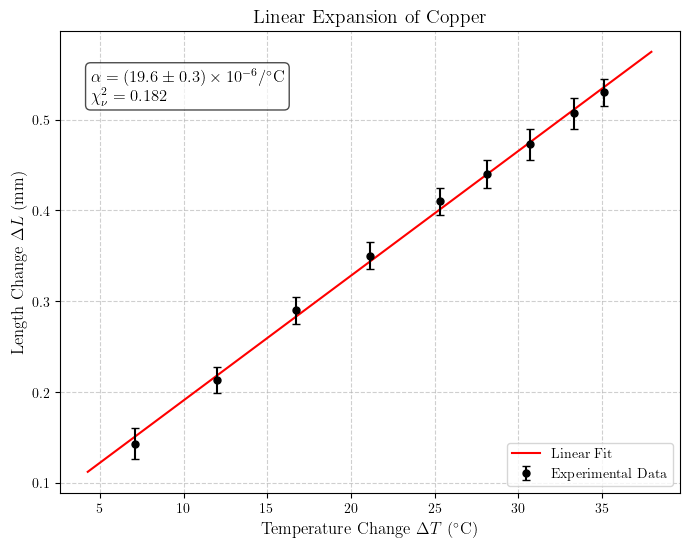
\includegraphics[width=1\textwidth]{CopperNoZero.png}
	\caption{กราฟแสดงความสัมพันธ์ระหว่างระยะยืด $\Delta L$ กับอุณหภูมิที่เปลี่ยนแปลงไป $\Delta T$ ของทองแดง}
    \label{fig:graph1}
\end{figure}

\bigskip

\begin{itemize}

    \item Chi-square (Reduced) Copper: $\chi_{\nu_{Cu}}^2 = 0.182$
    \medskip
    \item สัมประสิทธิ์การขยายตัวเชิงเส้นของทองแดง $\alpha_{Cu}$ ที่คำนวณได้: $\alpha_{Cu} = (19.6 \pm 0.3) \times 10^{-6} \ ^\circ\text{C}^{-1}$
    \medskip 
    \item สัมประสิทธิ์การขยายตัวเชิงเส้นของทองแดง $\alpha_{Cu}$ พร้อมค่าคาดเคลื่อนที่ปรับแล้ว (หารด้วย $\sqrt{\chi_{\nu_{Cu}}^2}$)\newline :  \mbox{$\alpha_{Cu} = (19.6 \pm 0.7) \times 10^{-6} \ ^\circ\text{C}^{-1}$}
    \medskip
    \item จุดตัดแกน $y$ พร้อมค่าคาดเคลื่อนที่ปรับแล้ว (หารด้วย $\sqrt{\chi_{\nu}^2}$): $c_{Cu} = 0.05 \pm 0.01$ mm

\end{itemize}

\newpage
\subsubsection*{การขยายตัวเชิงเส้นของเหล็กกล้า}

\begin{figure}[h]
	\centering
	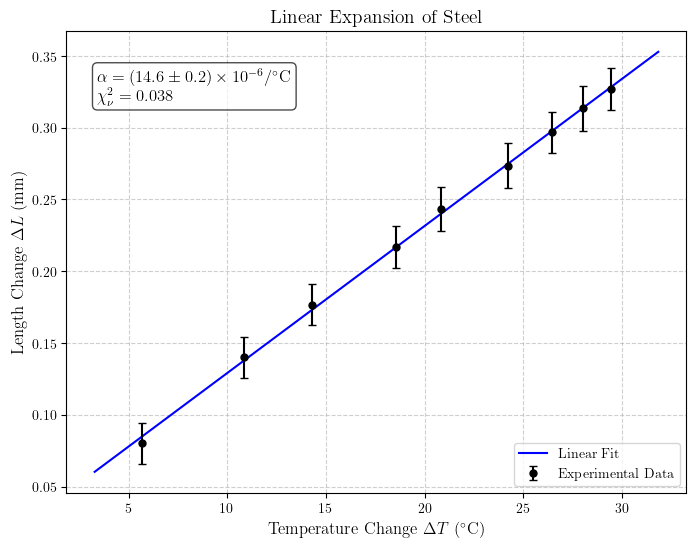
\includegraphics[width=1\textwidth]{SteelNoZero.png}
	\caption{กราฟแสดงความสัมพันธ์ระหว่างระยะยืด $\Delta L$ กับอุณหภูมิที่เปลี่ยนแปลงไป $\Delta T$ ของเหล็กกล้า}
    \label{fig:graph2}
\end{figure}

\bigskip

\begin{itemize}

    \item Chi-square (Reduced) Steel: $\chi_{\nu_{Steel}}^2 = 0.038$
    \medskip
    \item สัมประสิทธิ์การขยายตัวเชิงเส้นของเหล็กกล้า $\alpha_{Steel}$ ที่คำนวณได้: $\alpha_{Steel} = (14.6 \pm 0.2) \times 10^{-6} \ ^\circ\text{C}^{-1}$
    \medskip 
    \item สัมประสิทธิ์การขยายตัวเชิงเส้นของเหล็กกล้า $\alpha_{Steel}$ พร้อมค่าคาดเคลื่อนที่ปรับแล้ว (หารด้วย $\sqrt{\chi_{\nu_{Steel}}^2}$)\newline :  \mbox{$\alpha_{Steel} = (15 \pm 1) \times 10^{-6} \ ^\circ\text{C}^{-1}$}
    \medskip
    \item จุดตัดแกน $y$ พร้อมค่าคาดเคลื่อนที่ปรับแล้ว (หารด้วย $\sqrt{\chi_{\nu_{Steel}}^2}$): $c_{Steel} = 0.03 \pm 0.01$ mm

\end{itemize}

\newpage
\subsubsection*{การขยายตัวเชิงเส้นของอะลูมิเนียม}

\begin{figure}[h]
	\centering
	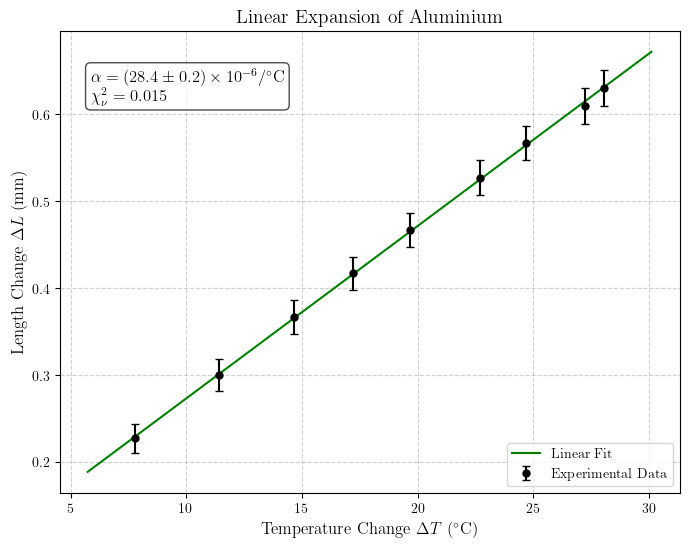
\includegraphics[width=1\textwidth]{AluminiumNoZero.png}
	\caption{กราฟแสดงความสัมพันธ์ระหว่างระยะยืด $\Delta L$ กับอุณหภูมิที่เปลี่ยนแปลงไป $\Delta T$ ของอะลูมิเนียม}
    \label{fig:graph3}
\end{figure}

\bigskip

\begin{itemize}

    \item Chi-square (Reduced) Aluminium: $\chi_{\nu_{Al}}^2 = 0.015$
    \medskip
    \item สัมประสิทธิ์การขยายตัวเชิงเส้นของอะลูมิเนียม $\alpha_{Al}$ ที่คำนวณได้: $\alpha_{Al} = (28.4 \pm 0.2) \times 10^{-6} \ ^\circ\text{C}^{-1}$
    \medskip 
    \item สัมประสิทธิ์การขยายตัวเชิงเส้นของอะลูมิเนียม $\alpha_{Al}$ พร้อมค่าคาดเคลื่อนที่ปรับแล้ว (หารด้วย $\sqrt{\chi_{\nu_{Al}}^2}$)\newline :  \mbox{$\alpha_{Al} = (28 \pm 2) \times 10^{-6} \ ^\circ\text{C}^{-1}$}
    \medskip
    \item จุดตัดแกน $y$ พร้อมค่าคาดเคลื่อนที่ปรับแล้ว (หารด้วย $\sqrt{\chi_{\nu_{Al}}^2}$): $c_{Al} = 0.07 \pm 0.02$ mm

\end{itemize}

จากการฟิตสมการเชิงเส้นพบว่ากราฟทั้งสามไม่ผ่านจุดกำเนิด โดยมีค่า $c_{Cu} = 0.05 \pm 0.01$ mm ค่า $c_{Steel} = 0.03 \pm 0.01$ mm และค่า $c_{Al} = 0.07 \pm 0.02$ mm แต่ค่าดังกล่าวเป็นค่าคงที่ซึ่งไม่ส่งผลกระทบต่อความชันของกราฟ ดังนั้นค่าความชันซึ่งนำไปคำนวณค่า $\alpha$ จึงยังคงมีความถูกต้องแม่นยำภายในขอบเขตของการทดลอง


\newpage
\section*{อภิปรายผล}

จากการทดลองนี้ ได้ทำการศึกษาความสัมพันธ์ระหว่างระยะยืดเฉลี่ยของแท่งโลหะ
$\Delta L$ และอุณหภูมิที่เปลี่ยนแปลง $\Delta T$ สำหรับโลหะสามชนิด ได้แก่
ทองแดง เหล็กกล้า และอะลูมิเนียม
โดยอุณหภูมิถูกคำนวณจากค่าความต้านทานของเทอร์มิสเตอร์ด้วยสมการ Steinhart--Hart
ซึ่งทำให้สามารถแปลงค่าความต้านทานเป็นอุณหภูมิได้อย่างต่อเนื่องและแม่นยำ

เมื่อพล็อตกราฟ $\Delta L$ กับ $\Delta T$ และทำการฟิตด้วยสมการเชิงเส้น
\[
\Delta L = \alpha L_0 \Delta T + c
\]
พบว่าข้อมูลของโลหะทั้งสามชนิดสามารถอธิบายได้ด้วยความสัมพันธ์เชิงเส้น
ซึ่งสอดคล้องกับทฤษฎีการขยายตัวเชิงเส้นของของแข็ง
โดยค่าสัมประสิทธิ์การขยายตัวเชิงเส้น $\alpha$ สามารถหาได้จากความชันของกราฟโดยตรง
\newline
\medskip

\textbf{ในกรณีของทองแดง} การฟิตกราฟให้ค่า
\[
\alpha_{Cu} = (19.6 \pm 0.3)\times10^{-6}\ ^\circ\mathrm{C}^{-1}
\]
และมีค่า reduced chi-square เท่ากับ
\[
\chi_{\nu_{Cu}}^2 = 0.182
\]
ซึ่งมีค่าน้อยกว่าหนึ่ง แสดงว่าความไม่แน่นอนของข้อมูลอาจถูกประเมินค่าสูงเกินจริง
เมื่อทำการปรับค่าความไม่แน่นอนโดยหารด้วย $\sqrt{\chi_{\nu_{Cu}}^2}$
จะได้ค่าที่ปรับแล้วเป็น
\[
\alpha_{Cu} = (19.6 \pm 0.7)\times10^{-6}\ ^\circ\mathrm{C}^{-1}
\]

\newline
\medskip

\textbf{ในกรณีของเหล็กกล้า} ได้ค่า
\[
\alpha_{Steel} = (14.6 \pm 0.2)\times10^{-6}\ ^\circ\mathrm{C}^{-1}
\]
โดยมีค่า reduced chi-square เท่ากับ
\[
\chi_{\nu_{Steel}}^2 = 0.062
\]
ซึ่งมีค่าน้อยกว่าหนึ่ง แสดงว่าความไม่แน่นอนของข้อมูลอาจถูกประเมินค่าสูงเกินจริง
เมื่อปรับค่าความไม่แน่นอนแล้วจะได้
\[
\alpha_{Steel} = (15 \pm 1)\times10^{-6}\ ^\circ\mathrm{C}^{-1}
\]

\newline
\medskip

\textbf{ในกรณีของอะลูมิเนียม} การฟิตกราฟให้ค่า
\[
\alpha_{Al} = (28.4 \pm 0.2)\times10^{-6}\ ^\circ\mathrm{C}^{-1}
\]
และมีค่า reduced chi-square เท่ากับ
\[
\chi_{\nu_{Al}}^2 = 0.015
\]
ซึ่งอยู่ใกล้เคียงหนึ่ง แสดงว่าการประเมินค่าความไม่แน่นอนมีความเหมาะสม
และเมื่อทำการปรับค่าความไม่แน่นอนแล้วได้
\[
\alpha_{Al} = (28 \pm 2)\times10^{-6}\ ^\circ\mathrm{C}^{-1}
\]

จากการฟิตกราฟพบว่าเส้นตรงของโลหะทั้งสามชนิดไม่ผ่านจุดกำเนิด
โดยมีค่า intercept เท่ากับ
\[
c_{Cu} = 0.05 \pm 0.01\ \mathrm{mm}, \quad
c_{Steel} = 0.03 \pm 0.01\ \mathrm{mm}, \quad
c_{Al} = 0.07 \pm 0.02\ \mathrm{mm}
\]
ซึ่งอาจเกิดจากความคลาดเคลื่อนเชิงระบบ
เช่น การตั้งศูนย์ของอุปกรณ์วัดระยะ การเสื่อมสภาพของ Thermistor
หรือการขยายตัวของส่วนประกอบอื่นในระบบทดลอง
อย่างไรก็ตาม ค่า intercept เหล่านี้ไม่ส่งผลต่อความชันของกราฟ
ดังนั้นค่าค่าสัมประสิทธิ์การขยายตัวเชิงเส้น $\alpha$
จึงยังคงมีความถูกต้องภายในขอบเขตของการทดลอง

เมื่อเปรียบเทียบค่าที่ได้จากการทดลอง
พบว่าลำดับขนาดของค่าสัมประสิทธิ์การขยายตัวเชิงเส้นเป็น
\[
\alpha_{\text{Al}} > \alpha_{\text{Cu}} > \alpha_{\text{Steel}}
\]
ซึ่งสอดคล้องกับพฤติกรรมทางกายภาพของโลหะ
เนื่องจากอะลูมิเนียมมีโครงสร้างผลึกที่ยอมให้ระยะระหว่างอะตอมเปลี่ยนแปลงได้ง่ายกว่า
ขณะที่เหล็กกล้ามีแรงยึดเหนี่ยวระหว่างอะตอมสูงกว่า
ทำให้มีการขยายตัวน้อยกว่าเมื่ออุณหภูมิเปลี่ยนแปลง

โดยรวมแล้ว การทดลองนี้สามารถแสดงให้เห็นความสัมพันธ์เชิงเส้นระหว่างการขยายตัวของโลหะกับอุณหภูมิได้อย่างชัดเจน
และค่าค่าสัมประสิทธิ์การขยายตัวเชิงเส้นที่ได้มีความสัมพันธ์ุทีสอดคล้องเมื่อเทียบกับค่าจากแหล่งอื่น
ความคลาดเคลื่อนหลักของการทดลองเกิดจากความไม่อุดมคติของระบบทดลองเช่น การเสื่อมสภาพของ Thermister การประมาณค่า $L_0$ ความไม่บริษุทธิ์ของโลหะ การประมาณค่าความไม่แน่นอน ข้อจำกัดของอุปกรณ์วัด และจำนวนข้อมูลที่น้อยเกินไป ซึ่งถือว่าอยู่ในระดับที่ยอมรับได้สำหรับการทดลองในครั้งนี้




\section{สรุป} \label{conclusion}

การทดลองนี้ได้ศึกษาการขยายตัวเชิงเส้นของโลหะสามชนิด ได้แก่ ทองแดง เหล็กกล้า และอะลูมิเนียม
โดยวัดความยาวที่เปลี่ยนไปของแท่งโลหะขณะอุณหภูมิเปลี่ยนแปลง
และคำนวณอุณหภูมิจากค่าความต้านทานของเทอร์มิสเตอร์ด้วยสมการ Steinhart--Hart
จากนั้นทำการฟิตกราฟความสัมพันธ์ระหว่าง $\Delta L$ และ $\Delta T$ ด้วยสมการเชิงเส้น

ค่าสัมประสิทธิ์การขยายตัวเชิงเส้นที่ได้จากการทดลอง (พร้อมค่าคาดเคลื่อนที่ปรับแล้ว)
สรุปได้ดังนี้
\begin{align*}
\alpha_{Cu} &= (19.6 \pm 0.7)\times10^{-6}\ ^\circ\mathrm{C}^{-1} \quad \text{(ทองแดง)} \\
\alpha_{Steel} &= (15 \pm 1)\times10^{-6}\ ^\circ\mathrm{C}^{-1} \quad \text{(เหล็กกล้า)} \\
\alpha_{Al} &= (28 \pm 1)\times10^{-6}\ ^\circ\mathrm{C}^{-1} \quad \text{(อะลูมิเนียม)}
\end{align*}

ผลการทดลองแสดงลำดับขนาดของค่าสัมประสิทธิ์การขยายตัวเชิงเส้นเป็น
\[
\alpha_{\text{Al}} > \alpha_{\text{Cu}} > \alpha_{\text{Steel}}
\]
ซึ่งสอดคล้องกับพฤติกรรมทางกายภาพของโลหะ
โดยกราฟที่ได้มีความเป็นเชิงเส้น และค่าความคลาดเคลื่อนอยู่ในระดับที่ยอมรับได้สำหรับชุดการทดลอง
สรุปได้ว่าการทดลองนี้สามารถอธิบายการขยายตัวเชิงเส้นของโลหะได้อย่างถูกต้องภายในขอบเขตของการทดลอง


\begin{thebibliography}{9}

\bibitem{Halliday}
David Halliday, Robert Resnick, and Jearl Walker,
\textit{Fundamentals of Physics},
10th Edition,
Wiley, 2013.

\bibitem{Taylor}
John R. Taylor,
\textit{An Introduction to Error Analysis: The Study of Uncertainties in Physical Measurements},
2nd Edition,
University Science Books, 1997.

\bibitem{SteinhartHart}
J. S. Steinhart and S. R. Hart,
“Calibration curves for thermistors,”
\textit{Deep Sea Research and Oceanographic Abstracts},
vol. 15, no. 4, pp. 497--503, 1968.

\bibitem{NIST}
National Institute of Standards and Technology (NIST),
“Thermal Expansion of Materials,”
Available: \url{https://www.nist.gov}

\bibitem{LMFIT}
Matthew Newville et al.,
“LMFIT: Non-Linear Least-Square Minimization and Curve-Fitting for Python,”
Available: \url{https://lmfit.github.io/lmfit-py/}

\bibitem{UT33B}
UNI-T,
\textit{UT33B+ Digital Multimeter User Manual},
UNI-T Technologies.

\end{thebibliography}

\end{document}
%